\documentclass[12pt]{article}
\usepackage{bbold}
\usepackage{amsfonts}
\usepackage{amsmath}
\usepackage{amssymb}
\usepackage{color}
\setlength{\columnseprule}{1pt}
\usepackage[utf8]{inputenc}
\usepackage[T2A]{fontenc}
\usepackage[english, russian]{babel}
\usepackage{graphicx}
\usepackage{hyperref}
\usepackage{mathdots}
\usepackage{xfrac}


\def\columnseprulecolor{\color{black}}

\graphicspath{ {./resources/} }


\usepackage{listings}
\usepackage{xcolor}
\definecolor{codegreen}{rgb}{0,0.6,0}
\definecolor{codegray}{rgb}{0.5,0.5,0.5}
\definecolor{codepurple}{rgb}{0.58,0,0.82}
\definecolor{backcolour}{rgb}{0.95,0.95,0.92}
\lstdefinestyle{mystyle}{
    backgroundcolor=\color{backcolour},   
    commentstyle=\color{codegreen},
    keywordstyle=\color{magenta},
    numberstyle=\tiny\color{codegray},
    stringstyle=\color{codepurple},
    basicstyle=\ttfamily\footnotesize,
    breakatwhitespace=false,         
    breaklines=true,                 
    captionpos=b,                    
    keepspaces=true,                 
    numbers=left,                    
    numbersep=5pt,                  
    showspaces=false,                
    showstringspaces=false,
    showtabs=false,                  
    tabsize=2
}

\lstset{extendedchars=\true}
\lstset{style=mystyle}

\newcommand\0{\mathbb{0}}
\newcommand{\eps}{\varepsilon}
\newcommand\overdot{\overset{\bullet}}
\DeclareMathOperator{\sign}{sign}
\DeclareMathOperator{\re}{Re}
\DeclareMathOperator{\im}{Im}
\DeclareMathOperator{\Arg}{Arg}
\DeclareMathOperator{\const}{const}
\DeclareMathOperator{\rg}{rg}
\DeclareMathOperator{\Span}{span}
\DeclareMathOperator{\alt}{alt}
\DeclareMathOperator{\Sim}{sim}
\DeclareMathOperator{\inv}{inv}
\DeclareMathOperator{\dist}{dist}
\newcommand\1{\mathbb{1}}
\newcommand\ul{\underline}
\renewcommand{\bf}{\textbf}
\renewcommand{\it}{\textit}
\newcommand\vect{\overrightarrow}
\newcommand{\nm}{\operatorname}
\DeclareMathOperator{\df}{d}
\DeclareMathOperator{\tr}{tr}
\newcommand{\bb}{\mathbb}
\newcommand{\lan}{\langle}
\newcommand{\ran}{\rangle}
\newcommand{\an}[2]{\lan #1, #2 \ran}
\newcommand{\fall}{\forall\,}
\newcommand{\ex}{\exists\,}
\newcommand{\lto}{\leftarrow}
\newcommand{\xlto}{\xleftarrow}
\newcommand{\rto}{\rightarrow}
\newcommand{\xrto}{\xrightarrow}
\newcommand{\uto}{\uparrow}
\newcommand{\dto}{\downarrow}
\newcommand{\lrto}{\leftrightarrow}
\newcommand{\llto}{\leftleftarrows}
\newcommand{\rrto}{\rightrightarrows}
\newcommand{\Lto}{\Leftarrow}
\newcommand{\Rto}{\Rightarrow}
\newcommand{\Uto}{\Uparrow}
\newcommand{\Dto}{\Downarrow}
\newcommand{\LRto}{\Leftrightarrow}
\newcommand{\Rset}{\bb{R}}
\newcommand{\Rex}{\overline{\bb{R}}}
\newcommand{\Cset}{\bb{C}}
\newcommand{\Nset}{\bb{N}}
\newcommand{\Qset}{\bb{Q}}
\newcommand{\Zset}{\bb{Z}}
\newcommand{\Bset}{\bb{B}}
\renewcommand{\ker}{\nm{Ker}}
\renewcommand{\span}{\nm{span}}
\newcommand{\Def}{\nm{def}}
\newcommand{\mc}{\mathcal}
\newcommand{\mcA}{\mc{A}}
\newcommand{\mcB}{\mc{B}}
\newcommand{\mcC}{\mc{C}}
\newcommand{\mcD}{\mc{D}}
\newcommand{\mcJ}{\mc{J}}
\newcommand{\mcT}{\mc{T}}
\newcommand{\us}{\underset}
\newcommand{\os}{\overset}
\newcommand{\ol}{\overline}
\newcommand{\ot}{\widetilde}
\newcommand{\vl}{\Biggr|}
\newcommand{\ub}[2]{\underbrace{#2}_{#1}}

\def\letus{%
    \mathord{\setbox0=\hbox{$\exists$}%
             \hbox{\kern 0.125\wd0%
                   \vbox to \ht0{%
                      \hrule width 0.75\wd0%
                      \vfill%
                      \hrule width 0.75\wd0}%
                   \vrule height \ht0%
                   \kern 0.125\wd0}%
           }%
}
\DeclareMathOperator*\dlim{\underline{lim}}
\DeclareMathOperator*\ulim{\overline{lim}}

\everymath{\displaystyle}

% Grath
\usepackage{tikz}
\usetikzlibrary{positioning}
\usetikzlibrary{decorations.pathmorphing}
\tikzset{snake/.style={decorate, decoration=snake}}
\tikzset{node/.style={circle, draw=black!60, fill=white!5, very thick, minimum size=7mm}}

\title{Дискретная математика. Теория}
\author{Александр Сергеев}
\date{}

\begin{document}
\maketitle
\section{Булевы функции}

\textit{Множество} - структура, связанная с своими элементами отношением принадлежности или непринадлежности.\\
\textit{(Не является определением)}\\\\
Элементы множества принадлежат некоторому универсуму $U$.\\\\
Операции над множествами:
\begin{enumerate}
    \item $A \cup B$ - Объединение
    \item $A \cap B$ - Пересечение
    \item $A \setminus B$ - Вычитание
    \item $A^c$ - Дополненте
    \item $A\ \triangle\ B;\quad A \oplus B$ - Исключающее объединение
    \item $A \times B$ - Декартово произведение
    \item $A^k$ - Декартова степень(вектор)
\end{enumerate}
Свойства декартова произведения:
\begin{enumerate}
    \item Можно считать, что $A \times A \times A = (A \times A) \times A = A \times (A \times A)$
    \item $A^0 = \{ () \} = void$
\end{enumerate}
Отношения множеств:
\begin{enumerate}
    \item $A \subset B$ - включает
    \item $A \subseteq B$ - включает или равно(эквивалентно первому в некоторых нотациях)
    \item $A = B$ - равенство
\end{enumerate}

\section{Отношения множеств. Бинарные отношения}
Бинарные отношения - множества пар элементов, которые находятся в отношениях.\\\\
Пусть $R$ - бинарное отношение.\\
$R \subset A \times B$\\\\
$a$ и $b$ находятся в отношении R $\Leftrightarrow (a,b) \in R \Leftrightarrow a\,R\,b$ \\\\
\textit{Полное отношение} - отношение $U^2$.\\\\
\textit{Парадокс Рассела(парадокс брадобрея):\\}
Пусть $A = \{ X: X \notin X\}$\\
Парадоксальность:\\
$A \in A \Rightarrow A \notin A$\\
$A \notin A \Rightarrow A \in A$\\
\section{Функции(Отношения)}
Функции $\subset$ Отношения\\
$B^A$ - множество функций из $A$ в $B$\\
$f \subset A \times B$\\\\
$\forall\ a \in A\quad\exists! b \in B: (a,b)\in f$ - функция(график)\\\\
\textit{(Комментарий к обозначению $B^A$: каждому элементу $A$ соответствует один из элементов $B$. Тогда одна функция задается одной парой из $B^{|A|}$)}\\\\
Инъекция: $x \neq y\ \Rightarrow f(x) \neq f(y)$\\
Сюръекция: $\forall y\ \exists x: f(x)=y$\\
Биекция = Инъекция $\land$ Сюръекция\\\\
Свойства отношений:
\begin{enumerate}
    \item $\forall a: a\,R\,a$ - Рефлексивные
    \item $\forall a: \overline{a\,R\,a}$ - Антирефлексивные
    \item $a\,R\,b\ \Rightarrow\ b\,R\,a$ - Симметричные
    \item если $a \neq b$, то $a\,R\,b\ \Rightarrow\ \overline{b\,R\,a}$ - Антисимметричные\\
    $a\,R\,b\ \land\ b\,R\,a\ \Rightarrow\ a=b$
    \item $a\,R\,b,\ b\,R\,c\ \Rightarrow\ a\,R\,c$ - Транзитивные
    \item Рефлексивное $\land$ Симметричное $\land$ Транзитивное = Отношение эквивалентности
    \item Рефлексивное $\land$ Антисимметричное $\land$ Транзитивное = Частичный порядок(Множество - частично упорядоченное множество/ч.у.м./p.o.set/poset. Линейный порядок - $\forall\,a,b\ a\,R\,b \lor b\,R\,a$)
\end{enumerate}
\textbf{Теорема}\\
Пусть $A$ - множество, $R$ - отношение эквивалентности на $A$.\\
Тогда $\exists$ множество $A/R$ классов эквивалентности: $A/R = \{ B | B$ - подмножество $A$ не пересекающееся$, x\,R\,y\ \Leftrightarrow\ \exists B \in A/R: x \in B \land y \in B\}$.\\\\
\textbf{Определение}\\
$R \subset A \times B\\
S \subset B \times C$\\
\textit{Композиция отношений} $T=R\circ S = RS: a\,T\,b \Leftrightarrow \exists c: a\,R\,c \land c\,S\,b\\
R^n = R\circ R^{n-1}; R^0=I\\
R^*=\bigcup_{k=0}^\infty R^k$ - рефлексивно-транзитивное замыкание\\
$R^+=\bigcup_{k=1}^\infty R^k$ - транзитивное замыкание\\\\
\textbf{Теорема}\\
Пусть $K$ - множество всех транзитивных отношений на $A$, содержащих $R$.\\
$\bigcap_{S\in K}S = \operatorname{TrCl} R$.\\
Тогда $\operatorname{TrCl} R = R^+$\\
\textbf{Доказательство}\\
Докажем $\operatorname{TrCl} R \subset R^+.\\
a R^+ b, b R^+ c \Rightarrow a R^i b, b R^j c \Rightarrow a R^{i+j} c \Rightarrow a R^+ c\\
R \subset R^+.$\\
Тогда $R^+ \in K \Rightarrow \operatorname{TrCl} R \subset R^+$\\
Докажем $R^+ \subset \operatorname{TrCl} R.\\
\forall S \in K, R^+ \subset S$\\
По индукции докажем $\forall\,k\geq 1\ R^k\subset S:$\\
\begin{enumerate}
    \item $R \subset S$
    \item $a R^{k+1} b \Rightarrow \exists\,c:\ a R^k c \land c R b \Rightarrow a S c \land c S b \Rightarrow a \S b$. Отсюда $R^{k+1} \subset S \Rightarrow \bigcup_{k=1}^\infty R^k \subset S \Rightarrow R^+ \subset S \Rightarrow R^+ \subset \bigcap_{S \in k} S$.
\end{enumerate}
Из 1 и 2 $\operatorname{TrCl} R = R^+$, ч.т.д.\\\\\\
\textbf{Определение}\\
\textit{Функциональное отношение} $R: R^TR=I$, где $I$ - отношение равенства.\\
\textit{Функциональное отношение} $R: a\,R\,b_1 \land a\,R\,b_2 \Leftrightarrow b_1 = b_2$.\\\\
\section{Булевы функции}
$\mathbb{B} = {0,1}\\
f: \mathbb{B}^n \rightarrow \mathbb{B}$ - $n$-арная булефа функция.\\\\
\subsection{Унарные функции}
$\mathbb{0}_n$ - тождественный 0: $\forall\,b_1,\ldots,b_n\ \mathbb{0}_n(b_1,\ldots,b_n) = 0$\\
$\mathbb{1}_n$ - тождественный 1: $\forall\,b_1,\ldots,b_n\ \mathbb{1}_n(b_1,\ldots,b_n) = 1$ \\
$\operatorname{id}$: $\forall\,b\ \operatorname{id}(b) = b$ \\
$\lnot$ - отрицание: $\forall\,b\ \lnot b = 1-b$
\subsection{Бинарные функции}
\begin{center}
    \begin{tabular}{c c| c c c c c c c c c c c c c c c c}
        $x$ & $y$ & $\mathbb{0}$ & $\land$ & $\nrightarrow$ & $x$ & $\nleftarrow$ & $y$ & $\oplus$ & $\lor$ & $\downarrow(\text{nor})$ & $\equiv$ & $\overline{y}$ & $\leftarrow$ & $\overline{x}$ & $\rightarrow$ & $\uparrow$ & $\mathbb{1}$\\
        \hline
        0 & 0 & 0 & 0 & 0 & 0 & 0 & 0 & 0 & 0 & 1 & 1 & 1 & 1 & 1 & 1 & 1 & 1\\
        0 & 1 & 0 & 0 & 0 & 0 & 1 & 1 & 1 & 1 & 0 & 0 & 0 & 0 & 1 & 1 & 1 & 1\\
        1 & 0 & 0 & 0 & 1 & 1 & 0 & 0 & 1 & 1 & 0 & 0 & 1 & 1 & 0 & 0 & 1 & 1\\
        1 & 1 & 0 & 1 & 0 & 1 & 0 & 1 & 0 & 1 & 0 & 1 & 0 & 1 & 0 & 1 & 0 & 1\\
    \end{tabular}
\end{center}

\subsection{Тернарные функции}
$<x\ y\ z>$ - медиана(возвращает 1 при 2 и более единицах)\\
$x\ ?\ y\ :\ z$ - переключатель
\subsection{Формулы}
\textbf{Определение}\\
\textit{Замыкание множества $A$} - множество функций, которые можно получить с помощью композиции и подстановки функций из $A$\\
\textbf{Определение}\\
\textit{Базис} или \textit{полная система связок} - система связок, с помощью которой можно задать любую функцию.\\\\
\textbf{Определение}\\
\textit{Канонический базис} - базис $\{\lor,\land,\lnot\}$\\\\
\textbf{Определение}\\
\textit{Совершенная дизъюнктивная нормальная формула} - формула, вида\\
$f(x_1, x_2, \ldots, x_n) = \ldots \lor \ldots \lor \ldots$, где мы добавляем $\ldots \land \lnot x_j \land \ldots \land x_i \land \ldots $ в формулу, если $f(\ldots, x_j = 0,\ldots, x_i = 1, \ldots) = 1$\\
\textbf{Определение}\\
Множество булевых функций $A$ полное, если любую булеву функцию $f$ можно выразить через элементы $A$.\\
\textbf{Лемма}\\
$A$ и $B$ - множество булевых функций.\\
$f$ можно выразить через $A$.\\
$\forall\,g\in A\ g$ можно выразить через $B$.\\
Тогда $f$ можно выразить через $B$.\\\\
\textbf{Следствие}\\
$A$ - базис.\\
$\forall\,\phi \in A\ \phi$ можно выразить через $B$.\\
Тогда $B$ - базис.
\subsection{Классы Поста}
\begin{enumerate}
    \item $F_0$ - сохраняющие 0. $\{f\,|\,f(0,\ldots,0) = 0\}$
    \item $F_1$ - сохраняющие 1. $\{f\,|\,f(1,\ldots,1) = 1\}$
    \item $F_s$ - самодвойственные функции. $\{f\,|\,\lnot f(\lnot x_1,\ldots,\lnot x_n) = f(x_1,\ldots,x_n)\}$
    \item $F_m$ - монотонные функции. $\{f\,|(\,\forall\,i\ x_i \leq y_i )\Rightarrow f(x_1,\ldots, x_n) \leq f(y_1,\ldots, y_n)\}$
    \item $F_l$ - линейная функция. $\{ f\,|\, f - \oplus$ от некоторых $x_i$ и $\mathbb{1} \}$
\end{enumerate}
Если все функции $A$ принадлежат к некому классу поста $F_*$, то все функции, которые можно выразить через $A$, принадлежат $F_*$\\\\
\textbf{Определение}\\
Запись функции через $\{\oplus,\land,\mathbb{1}\}$ - \textit{Полином Жегалкина}.\\
Запись xor-ов конъюнкций - \textit{Канонический вид полинома Жегалкина}.\\\\
\textbf{Теорема}\\
У любой булевой функции, кроме тождественного нуля, существует единственный канонический полином Жегалкина.\\
\textbf{Доказательство}\\
Он существует, т.к. $\{\oplus,\land,\mathbb{1}\}$ - базис.\\
Слагаемых $2^n$ от количества аргументов $n$. Каждое слагаемое может входить или не входить в полином. Тогда канонических полиномов Жегалкина $2^{2^n}$, включая пустой. Всего булевых функций тоже $2^{2^n}$. Тогда между полиномами Жигалкина и булевыми функциями  биекция, ч.т.д.\\\\
\textbf{Теорема(Поста о полной системе функций)}\\
Пусть $A \nsubseteq F_0,F_1,F_s,F_l,F_m$. Тогда $A$ - базис.\\
\textbf{Доказательство}\\
Пусть $f_0(0,\ldots,0) = 1$.
\begin{enumerate}
    \item $f_0(1,\ldots,1) = 1$\\
    $f_0(x,\ldots,x) = \mathbb{1}$
    \item $f_0(1,\ldots,1) = 0$\\
    $f_0(x,\ldots,x) = \lnot x$
\end{enumerate}
Пусть $f_1(1,\ldots,1) = 0$.
\begin{enumerate}
    \item $f_1(0,\ldots,0) = 0$\\
    $f_1(x,\ldots,x) = \mathbb{0}$
    \item $f_1(0,\ldots,0) = 0$\\
    $f_1(x,\ldots,x) = \lnot x$
\end{enumerate}
Тогда по случаям:
\begin{enumerate}
    \item[аа.] $\mathbb{1},\mathbb{0}$\\
    Если $f_m$ не монотонная.\\
    Пусть $x_i\leq y_i$.\\
    Тогда $f_m(x_0,\ldots,x_n) = 1\\
    f_m(y_0,\ldots,y_n)=0$\\
    Будем постепенно заменять $x_i$ на $y_i$, начиная с 1 и до n. В какой-то момент функция сменит значение с 1 на 0. Тогда есть случай, когда \\
    $f_m(y_1,y_2,\ldots, y_{i-1}, x_i, x_{i+1}, \dots, x_n) = 1$\\
    $f_m(y_1,y_2,\ldots, y_{i-1}, y_i, x_{i+1}, \dots, x_n) = 0$.\\
    Тогда возьмем функцию $\lnot a = f_m(y_1,y_2,\ldots, y_{i-1}, a, x_{i+1}, \dots, x_n)$, взяв $y_1\ldots y_{i-1}$ и $x_{i+1}\ldots x_n$ в качестве констант
    \item[аб.] $\mathbb{1},\lnot,\mathbb{0}=\lnot\mathbb{1}$
    \item[ба.] $\mathbb{0},\lnot,\mathbb{1}=\lnot\mathbb{0}$
    \item[бб.] $\lnot$\\
    Пусть $f_s(x_1,\ldots,x_n) = f_s(\lnot x_1, \ldots, \lnot x_n)$ - не самодвойственная функция.\\
    Тогда найдем нарушение самодвойственности. К примеру, $f_s(0,0,1,1,0) = f_s(1,1,0,0,1)$.
    Тогда $f_s(\lnot x, \lnot x, x, x, \lnot x) = const$. Тогда мы получили $\mathbb{0}$ или $\mathbb{1}$, а через $\lnot$ и второе.
\end{enumerate}
Далее. Возьмем нелинейную функцию $f_l(x,y,\ldots)$ и представим ее в виде полинома Жегалкина. По теореме такой полином единственный, а из нелинейности следует, что хотя бы один член имеет не менее двух аргументов. Выберем минимальный член с не менее 2 аргументами. Выберем первые два члена в нем. Остальные аргументы приравняем к $\mathbb{1}$, а те, что не вошли - приравняем к $\mathbb{0}$.
Тогда мы получим один из вариантов
\begin{enumerate}
    \item $x\land y$. Тогда $f(x,y,\ldots)$ - искомый "И".
    \item $(x\land y) \oplus \mathbb{1}$. Тогда $\lnot f(x,y,\ldots)$ - искомый "И".
    \item $(x\land y) \oplus x = x\land(y\oplus \mathbb{1})$. Тогда $f(x,\lnot y,\ldots)$ - искомый "И".
    \item $(x\land y) \oplus y = y\land(x\oplus \mathbb{1})$. Тогда $f(\lnot x,y,\ldots)$ - искомый "И".
    \item $(x\land y) \oplus x \oplus y = x \lor y$. Тогда $f(x,y,\ldots)$ - искомый "ИЛИ".
    \item[$\ldots$]
\end{enumerate}
Имея $\{\land,\lnot\}$ или $\{\lor,\lnot\}$, можно получить канонический базис.\\
Отсюда ч.т.д.\\\\
\textbf{Определение}\\
$f$ - \textit{инволюция}, если $f = f^{-1} $
\subsection{Схема их функциональных элементов}
\textbf{Теорема о топологической сортировке}\\
В ацикличном ориентированном графе существует нумерация, при которой вершины с меньшими номерами ведут только в вершины с большими номерами\\
\textbf{Лемма}\\
В таком графе существует вершина, из которой не выходят ребра.\\
\textbf{Доказательство теоремы}\\
Докажем по индукции:
\begin{enumerate}
    \item Для $n=1$ верно
    \item Для $n > 1$:\\
    Рассмотрим $n-1$ вершину, исключая одну такую, из которой не выходят ребра. Пронумеруем их от $1$ до $n-1$ в соответствии с утверждением. Добавим удаленную вершину, присвоив ей номер $n$. Из нее не выходят вершин и ее номер наибольший. Тогда утверждение верно, ч.т.д.
\end{enumerate}
\textbf{Определение}\\
Выберем базис связок $F$\\ 
\textit{Схема из функциональных элементов} - это ацикличный ориентированный граф с кратными ребрами, в котором каждые входящие в вершину ребра пронумерованы.\\\\
СФЭ позволяют строить схемы функций.\\
Изначально у нас есть вершины $x_1,\ldots,x_n$ - аргументы нашей функции. Из аргументов идут ребра к вершинам, символизирующим функции из нашего базиса $F$(порядок входа ребер важен, количество входящих ребер соответствует количеству аргументов функции). Далее из любых вершин еще могут выходить ребра. Результат нашей функции символизируется одной из перечисленных вершин.\\\\
\textbf{Теорема}\\
Любую функцию можно задать СФЭ.\\
\textbf{Доказательство}\\
СФЭ - дерево разбора, направленное снизу вверх с объединением листьев в $n$ вершин.\\\\
Пусть $\operatorname{size}_A f$ - минимальное количество внутренних элементов СФЭ в схеме для $f$ над базисом $A$.\\
\textbf{Теорема}\\
Пусть $A$, $B$ - базисы\\
Тогда $\exists\,C\ \forall\,f\ \operatorname{size}_A f \leq C\cdot\operatorname{size}_B f$\\
\textbf{Доказательство}\\
Построим СФЭ функции $f$ в базисе $B$. Выразим все функции из $B$ через $A$. Пусть $C$ - максимальное количество элементов, которое мы использовали на одну функцию из $B$. Тогда одна вершина в исходной СФЭ заменилась не более чем на $C$. Тогда мы получили СФЭ из не менее $C\cdot\operatorname{size}_B f$. Тогда $\operatorname{size}_A f \leq C\cdot\operatorname{size}_B f$, ч.т.д. \\
\textbf{Определение}\\
\textit{Глубина схемы} - максимальная длина пути в СФЭ.\\\\
Пусть $\operatorname{depth}_A f$ - минимальная глубина СФЭ в схеме для $f$ над базисом $A$.\\
\textbf{Теорема}\\
Пусть $A$, $B$ - базисы\\
Тогда $\exists\,C\ \forall\,f\ \operatorname{depth}_A f \leq C\cdot\operatorname{depth}_B f$\\
\subsection{Минутка АрхЭВМ}
\subsubsection{Линейный сумматор}
\textit{Полусумматор} - $f(x_1, x_2) = (carry = x_1 \land x_2, sum = x_1 \oplus x_2)$\\
\textit{Полный сумматор} - $f(x_1, x_2, x_3) = (carry = \langle x_1 x_2 x_3 \rangle, sum = x_1 \oplus x_2 \oplus x_3)$\\
\textit{Линейный сумматор} двоичных чисел можно построить каскадом сумматоров.\\
Размер - $O(n)$, глубина - $\Omega(n)$\\\\
\subsubsection{Двоичный каскадный сумматор}
Рассмотрим $f_i: c_{i+1} = f_i(c_i)$\\
\begin{center}
    \begin{tabular}{c|c|c}
        $x$ & $y$ & $f$ \\
        \hline
        $0$ & $0$ & $\mathbb{0}$ = k(kill)\\
        $0$ & $1$ & $\operatorname{id}$ = p(propagate)\\
        $1$ & $0$ & $\operatorname{id}$ = p(propagate)\\
        $1$ & $1$ & $\mathbb{1}$ = g(generate)
    \end{tabular}
\end{center}
Рассмотри $f_1(f_2(x))$(столбец - $f_1$, строка $f_2$):
\begin{center}
    \begin{tabular}{c|c c c}
        f & k & g & p \\\hline
        k & k & g & k \\
        g & k & g & g \\
        p & k & g & p
    \end{tabular}
\end{center}
Отсюда \\
$\begin{array}{ccc}
    \ldots k p p \ldots p & = & k\\
    \ldots g p p \ldots p & = & g\\
    p p p \ldots \ldots p & = & p\\
\end{array}$\\\\
Пусть количество аргументов $n=2^m$\\
Построим двоичное полное дерево, которое отвечает за определенное количество битов.\\
Корень:\\
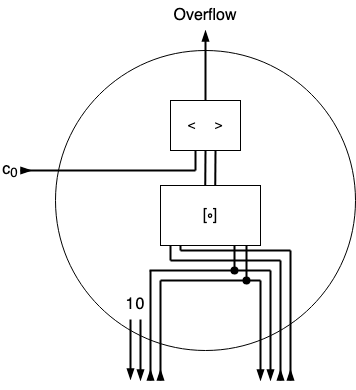
\includegraphics[height=10cm]{Root}\\
Лист:\\
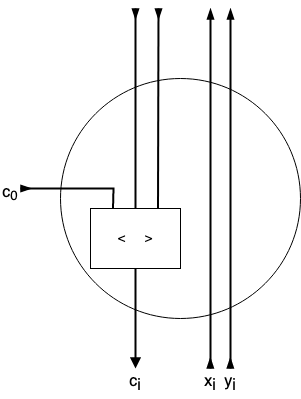
\includegraphics[height=10cm]{Leaf}\\
Узел:\\
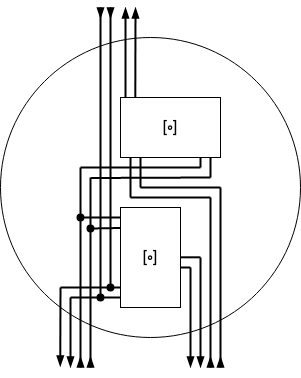
\includegraphics[height=10cm]{Node}\\
Здесь $[\circ]$ является блоком композиции, работающим по таблице выше. Нетрудно заметить, что в итоге на $i$-ый лист поступит композиция функций вида $f_{i-1} \circ f_{i-2} \circ \ldots \circ f_0$\\
Тогда на выходах листьев мы получим $c_0\ldots c_{n-1}$. В корне же мы получим параметр Overflow, указывающий, произошло ли переполнение\\
Сложив каждый $c_i$ с $x_i$ и $y_i$, мы получим искомую сумму\\
Количество вершин $2n-1=O(n)$\\
Глубина $O(\log n)$\\
\subsubsection{Вычитание}
Чтобы выполнить вычитание $x$ и $y$, нужно сделать сложение $x+\overline{y}+1$. Сложим $x$ и $\overline{y}$, подав $1$ на $c_0$ 
\subsubsection{Умножение}
Будем выполнять умножение первого числа на каждый разряд второго. В сумме блок, выполняющий это действие, будет иметь
размер $O(n^2)$, и глубину $O(1)$\\
Теперь научимся складывать имеющиеся $n$ чисел\\
Сумматор 3 в 2 - устройство, сопоставляющее числам $x$, $y$, $z$ числа $u$ и $v$ так, что $x+y+z=v+u$ и имеющее размер $O(n)$ и глубину $O(1)$. Таким сумматором является полный сумматор\\
\textit{Дерево Уоллеса}\\
Циклически будем подавать тройки значений на сумматоры 3 в 2, получив в результате два числа, которые сложим\\
Размер - $O(n^2)$\\
Глубина - $O(\log n)$\\\\
В итоге мы получаем схему умножения $x$ на $y$:\\
Первый блок генерирует $n$ чисел вида $x \land y_i << i$, которые суммируем деревом Уоллеса\\
Суммарный размер $O(n^2)$, глубина $O(\log n)$
\subsection{Оценка размера представления функции}
\textbf{Теорема}\\
Для любой булевой функции от $n$ аргументов достаточно $O(\frac{2^n}n)$\\
или\\
Для любого базиса $\exists\,C\ \forall\,0 < \varepsilon < 1\ \exists\,n_0:$ если $n>n_0$ и используется $<C\cdot\frac {2^n}n$ функциональных элементов, то можно реализовать $\leq \varepsilon\cdot 2^{2^n}$ функций\\
\textbf{Доказательство}\\
Выберем базис $B=\{\downarrow\}$\\
Рассмотрим линейную программу и рассмотрим сколько программ мы можем сделать\\
$\begin{array}{cc}
    x_{n+1}=x_{i_1}\downarrow x{j_1} & n^2 \text{способов}\\
    x_{n+2}=x_{i_2}\downarrow x{j_2} & (n+1)^2 \text{способов}\\
    \vdots & \vdots\\
    x_{n+k}=x_{i_k}\downarrow x{j_k} & (n+k)^2 \text{способов}\\
\end{array}$\\
Тогда количество функций $\leq$ число программ $\prod_{i=1}^k(n+i-1)^2 \leq (n+k)^{2k} = 2^{2k\log_2 (n+k)}\leq 2^{3C\cdot 2^n} \overset{*}{=} (2^{2^n})^{3C}$\\
(*) Пусть $k=C\frac{2^n}{n}$\\
$2k\log_2 (n+k) = \frac{2C\cdot 2^n}{n}\log_2(n+\frac{C\cdot 2^n}{n})\leq \frac{2C\cdot 2^n}{n}log_2(C\cdot 2^n)=\frac{2C\cdot 2^n(\log_2 C+n)}n = \frac{d\cdot 2^n}n+2c\cdot 2^n \leq 3C\cdot 2^n$\\(т.к. $\frac dn \rightarrow 0$)\\
Доля функций, которые можно реализовать за менее $O(\frac {2^n}n)$, стремится к 0\\
Теперь докажем, что $C\cdot \frac{2^n}n$ достаточно для большинства функций\\
Рассмотрим $s-k$-разложение Лупанова\\
Пусть у нас есть функция от $n$ аргументов\\
Назовем аргументы: $f(x_1,\ldots,x_k,y_1,\ldots,y_{n-k})$\\
Построим прямоугольную таблицу истинности:
\begin{center}
    \begin{tabular}{c|cccc}
        & $0\ldots00$ & $0\ldots01$ & $\cdots$ & $1\ldots11$\\
        \hline
        $0\ldots00$ & & & & \\
        $0\ldots01$ & & & & \\
        $\vdots$ & & & & \\
        $1\ldots11$ & & & &
    \end{tabular}
\end{center}
Нарежем таблицу на горизонтальные полосы ширины $s$. Всего их $p=\left\lceil \frac {2^n}s \right\rceil$\\
Теперь обнулим все полосы, кроме $i$-ой. Всего мы можем получить $p\cdot 2^s$ функций(т.к. не более $2^s$ вариантов столца высоты $s$). Назовем такие функции $g_{i,mask}$, где $mask$ - значения\\
$f(x_1,\ldots,x_k,y_1,\ldots,y_{n-k})=\bigvee_{i=1}^p g_{i,mask[y_1,\ldots,y_{n-k}]}(x_1,\ldots,x_k)$\\
Возьмем демультиплексор, адресом для которого будут выступать $x_1\ldots x_k$. На вход ему подадим единицу. Каждый выход будет соответствовать одной строчке в нашей таблице. Тогда 1 будет только на том выходе, которому соответствуют наши $x_1\ldots x_k$. На такой демультиплексор уйдет $2^k$ элементов. Далее для каждой полосы соберем все возможные функции $g$, взяв or от всех строк данной полосы, на которых $g$ равна 1. На одну такую функцию уйдет не более $s$ операций or. Всего таких функций $2^s$ на одну полосу, а полос $\frac{2^k}s$. Итого на все это уйдет $s2^s\frac{2^k}s = 2^{s+k}$. Далее для каждого набора $y_1\ldots y_{n-k}$ объединим все $g$ в один блок через or, которые соответствуют данному набору. Всего наборов $2^{n-k}$, а $g$ - $\frac{2^k}s$. Отсюда на этот фрагмент уйдет $\frac{2^n}s$ элементов. Потом с помощью мультиплексора, где адресом будет $y_1\ldots y_{n-k}$, выберем нужный нам набор. На это уйдет $2^{n-k}$ элементов.\\
Обобщая:
\begin{enumerate}
    \item Подадим 1 на выход демультиплексора, соответствующей строке $x_1\ldots x_k$
    \item Для каждой полосы $i$ создадим функцию $g_{i,m}$ для всех возможных уникальных $m$
    \item Для каждого набора $y_1\ldots y_{n-k}$ объединим все функции $g_{*,m}: m = mask[y_1\ldots y_{n-k}]$
    \item Через мультиплексор выберем среди всех объединений то, что соответствует нашим $y_1\ldots y_{n-k}$
\end{enumerate}
Итого мы можем собрать схему за $2^k+2^{s+k}+\frac{2^n}s+2^{n-k}$\\
Выберем $\left\{\begin{array}{l}
    k = 2\log_2 n  \\
    s = n - 3\log_2 n
\end{array}\right.$\\
Тогда $\left\{\begin{array}{l}
     2^k=n^2  \\\\
     2^{s+k} = \frac{2^n}{n}\\\\
     \frac{2^n}s\geq \frac{2\cdot 2^n}{n}\\\\
     2^{n-k} = \frac{2^n}{n^2}
\end{array}\right.$\\
Тогда суммарная асимптотика $O(\frac {2^n}n)$, ч.т.д.\\
Т.о. за такую асимптотику точно возможно реализовать функцию.\\
Объединяя обе теоремы, получаем, что для большинства функций $\operatorname{size} f = \Theta(\frac{2^n}n)$
\section{Представление информации}
\subsection{Код. Код Хаффмана. Неравенство Крафта-Макмилана}
\textbf{Определение}\\
\textit{Алфавит} - произвольное конечное непустое множество (обозначаются $\Sigma$)\\
\textit{Буква} или \textit{Символ} - элементы этого множества (обозначаются $a,b,c,\ldots$)\\
\textit{Множество слов над алфавитом $\Sigma$} или \textit{цепочка} или \textit{строка} - $\sum_{i=0}^\infty\ \Sigma^i$ (обозначают $u,v,w,x,y,z$ или $\alpha, \beta, \gamma, \ldots$)\\
Конкатенация $\cdot: \Sigma^*\times\Sigma^* \rightarrow \Sigma^*$ - получение строки путем приписывания второго операнда к концу первого\\
\textbf{Свойства конкатенации}
\begin{enumerate}
    \item $(\alpha\beta)\gamma = \alpha(\beta\gamma) = \alpha\beta\gamma$
    \item $\exists\,\varepsilon \in \Sigma^0:\ \alpha\varepsilon = \varepsilon\alpha=\alpha$ - нейтральный элемент
\end{enumerate}
Множество $(\Sigma, \cdot)$ - \textit{моноид} (на самом деле даже \textit{свободный} моноид над $\Sigma$)\\
$c$ - \textit{код} над $\Sigma$, если существует $c: U\rightarrow \Sigma^*$\\
Код \textit{однозначно декодируемый}, если $c$ - биекция\\
Если $U = \Pi^*$:\\
Тогда $c:\Pi^*\rightarrow \Sigma^*$\\
Код разделяемый, если $c$ - гомоморфизм(т.е. $c(\alpha\cdot\beta) = c(\alpha)\cdot c(\beta))$\\\\
Если код - однозначно декодируемый бинарный код постоянной длины:\\
$|c(a\in \Pi)| = \lceil \log_2 |\Pi| \rceil$\\\\
Теперь попробуем сделать код непостоянной длины\\
Пусть $f:\Pi \rightarrow \mathbb{N}$ - частота появления каждой буквы алфавита $\Pi$ в неком тексте\\
Минимизируем $\sum_{a\in\Pi} f(a)|c(a)| = \sum_{a\in\Pi} f(a)l(a)$ для данного текста, где $l(a)=|c(a)|$\\
\textit{Код Хаффмана} - оптимальный префиксный бинарный код\\
\textbf{Определение}\\
Код называется \textit{префиксным}, если $a \neq b \Rightarrow c(a)$ - не префикс $c(b)$\\
\textbf{Лемма}\\
Префиксный код однозначно декодируемый\\
\textbf{Доказательство}\\
Пусть это не так.
Тогда $\exists\,\alpha\beta\in \Pi^*:\ c(\alpha)=c(\beta)$\\
Пусть строчки различаются с $i$-ого символа. $c(\alpha_i)$ - префикс $c(\beta_i)$ или наоборот, что противоречит условию, ч.т.д.\\\\
\textbf{Неравенство Крафта-Макмилана}\\
Однозначно декодируемый разделяемый бинарный код с длинами слов $l_1,l_2,\ldots,l_n$ существует $\Leftrightarrow \sum_{i=1}^n 2^{-l_i} \leq 1$\\
\textbf{Доказательство $\Leftrightarrow$}\\
Следует из Леммы\\
\textbf{Доказательство $\Rightarrow$}\\
Доказать: если код однозначно декодируемый $\Rightarrow \sum_{i}2^{-l_i} \leq 1$\\
Выберем $\Pi = \{a,b\}$\\
Выберем кодовые слова $\alpha_1, \alpha_2,\ldots,\alpha_n$, являющиеся однозначно декодируемые\\
Рассмотрим полукольцо над словами\\
Сложим слова $S=\alpha_1+\alpha_2+\ldots+\alpha_n$ и возведем в $k$-ую степень\\
$S^k=(\alpha_1+\alpha_2+\ldots+\alpha_n)^k$\\
Мы получили сумму $n^k$ различных произведений (конкатенаций). Никакие два члена не равны из однозначности декодируемости\\
Пусть $a=b=\frac12$\\
Тогда $\alpha_1+\alpha_2+\ldots+\alpha_n = \sum_{i=1}^n (\frac12)^{l_i}$, где $l_i$ - длина $\alpha_i$\\
Длины всех всех произведений от $k$ (как минимум) до $Lk: L = \max_i l_i$\\
Сгруппируем все произведения длины $k$. Их количество $\leq 2^k$, а каждый член произведения равен $\frac1{2^k}$. Тогда сумма каждой группы не больше $1$\\
Отсюда $S^k \leq Lk$\\
Но $S = \sum_{i=1}^n 2^{-l_i}$\\
Тогда $\forall\,k\ (\sum_{i=1}^n 2^{-l_i})^k \leq Lk$\\
Если $S > 1$, то с некоторого места $S^k > Lk$\\
Отсюда $S \leq 1 \Leftrightarrow \sum_{i=1}^n 2^{-l_i} \leq 1$, ч.т.д.\\
\textbf{Лемма}\\
$\sum_{i=1}^n 2^{-l_i} \leq 1\Rightarrow$ существует оптимальный \underline{префиксный} код с длинами $l_1,\ldots,l_n$\\
\textbf{Доказательство}\\
Упорядочим $l_i: l_1 \leq l_2 \leq \ldots \leq l_n$\\
Возьмем отрезок длины 1 и последовательно отложим слева отрезки длин $2^{-l_i}$\\
Утверждается, что если сумма длин отрезков больше $\frac12$, то точка $\frac12$ на отрезке - граница какого-то отрезка\\
Доказем это:\\
Выберем отрезок $j$ такой, что\\
$2^{-l_1}+2^{-l_2}+\ldots+2^{-l_j} \leq \frac12$\\
$2^{-l_1}+2^{-l_2}+\ldots+2^{-l_j}+2^{-l_{j+1}} > \frac12$\\
Домножим оба выражения на $2^{l_{i+1}}$\\
Отсюда\\
$2^{l_{j+1}-l_1}+2^{l_{j+1}-l_2}+\ldots+2^{l_{j+1}-l_j} \leq 2^{l_{j+1}-1}$\\
$2^{l_{j+1}-l_1}+2^{l_{j+1}-l_2}+\ldots+2^{l_{j+1}-l_j}+1>2^{l_{j+1}-1}$\\
В обоих выражениях обе части целые. Из этого следует, что в первом выражении равенство, отсюда утверждение доказано\\
Теперь разделим отрезок пополам. Пусть коды в левой половине отрезка начинаются с 0, а в правой - с единицы\\
Тогда задача сводится к построению префиксного кода длин $l_i-1$ для левой и правой частей отдельно\\
Т.о. мы построили префиксный код, т.е. лемма доказана\\
\textbf{Лемма 1}\\
Существует оптимальное дерево, в котором $x,y: f_x,f_y$ минимальные --- братья на максимальной глубине\\
\textbf{Доказательство}\\
Рассмотрим вершину $a$ на максимальной глубине. 
\begin{enumerate}
    \item У нее есть брат $b$: если бы его не было, дерево было бы неоптимальным
    \item если $a,b$ имеют не минимальные $f_a,f_b$: поменяем местами $a,b$ местами с $x,y$, имеющими минимальные $f_x,f_y$. Тогда сумма $\sum_{a\in\Pi} f(a)l(a)$ не увеличится (к примеру, по перестановочному неравенству), а значит мы получим оптимальное дерево. Отсюда такое дерево существует
\end{enumerate}
\textbf{Алгоритм Хаффмана}\\
$\Pi = \{a_1,a_2,\ldots,a_n\}$\\
Построим \textit{бор} - дерево префиксного кода (в вершине хранится буква. Лист соответствует строке, полученной конкатенацией всех символов от корня до данного листа)\\
\begin{enumerate}
    \item Для $n = 2$ оптимальный бор - дерево из корня и двух листов
    \item Для $n > 2$:
    Выберем $x,y$ - два символа с минимальными $f_x$ и $f_y$\\
    Заменим их на символ $z$\\
    $f_z = f_x + f_y$\\
    Мы получили алфавит $\Pi'$. Решим для него задачу построения минимального кода с суммой $\Phi'$. Затем сделаем замену $c(x) = c(z)\cdot0, c(y) = c(z)\cdot1$\\
    После замены мы получили сумму\\
    $\Phi' = \sum_{a\in\Pi\setminus \{x,y\}} f(a)l(a) + f_zl_z = \sum_{a\in\Pi\setminus \{x,y\}} f(a)l(a) + (f_x+f_y)(l_x-1) = \sum_{a\in\Pi\setminus \{x,y\}} f(a)l(a) + f_xl_x+f_yl_y - (f_x+f_y) = \Phi - (f_x+f_y)$, где $\Phi$ - сумма для $n$ элементов\\
    Отсюда $\Phi = \Phi'+f_x+f_y$\\
    Т.к. $\Phi'$ - минимальное по индукционному переходу(сумма для кода из $n-1$ элементов), а $f_x, f_y$ - по условию, то $\Phi$ -  минимальное
\end{enumerate}
\subsection{Арифметическое кодирование}
\textbf{Кодирование}\\
Возьмем слово $S$. Посчитаем количество вхождений каждого символа в нем\\
Возьмем определенный порядок $a,b,c,\ldots$ символов в алфавите\\
Возьмем отрезок длины 1 и поделим его в отношении количества вхождений $f_a, f_b, f_c,\ldots$\\
Возьмем подотрезок, соответствующий $S_1$, и проделаем с ним ту же операцию\\
В данном подотрезке возьмем подотрезок, соответствующий $S_2$, и сделаем то же самое\\
Проделаем это последовательно для всех символов $S_i$\\
В последнем отрезке выберем точку $\frac{p}{2^q}$ с минимальным $q$\\
Тогда кодом данного слова будет бинарный код длины $2^q$ со значением $p$\\
\textbf{Декодирование}\\
Зная порядок $a,b,c,\ldots$ и отношение $C_a:C_b:C_c:\ldots$, будет разбивать отрезок длины $1$ в отношении $f_a:f_b:f_c:\ldots$ и определять, какому отрезку принадлежит $\frac{p}{2^q}$\\
Проделав такую операцию $|C_a+C_b+C_c+\ldots|$ раз, получим значение слова $S$\\
\textbf{Оценка}\\
Оценим длину результирующего отрезка\\
Пусть $C(S)$ - код\\
$\operatorname{len} C(S) = q$\\
Заметим, что $q = \lceil -\log_2 R-L \rceil$ точно подойдет\\
Тогда $q \leq \lceil -\log_2 R-L \rceil$\\
$R-L = 1\cdot\frac{f_{S_1}}{m}\cdot\frac{f_{S_2}}{m}\cdot\ldots = \frac{\prod_{i=1}^n f_i^{f_i}}{m^m}$, где $m = |S|$\\
$R-L = \frac{\prod_{i=1}^n f_i^{f_i}}{m^m} = \sum_{i=1}^n f_i\log_2 f_i - m\log_2 m = \sum_{i=1}^n f_i\log_2 f_ - \sum_{i=1}^n f_i log_2 m = m\sum_{i=1}^n \frac{f_i}{m}\log_2\frac{f_i}{m}$\\
$p_i = \frac{f_i}m$ - вероятность вхождения\\
$R-L = m\sum_{i=1}^n p_i\log_2 p_i$\\
$q \leq m\sum_{i=1}^n p_i\log_2 \frac1{p_i} = m\cdot H(p_1,\ldots,p_n)$
\subsection{Алгоритмы семейства LZ}
Разделим токены на 2 типа: символы и ссылки $(d_i, f_i)$ - повтори повтори последние $d_i$ повторяя их, выпиши $f_i$ символов\\
*TODO*
\subsubsection{LZW}
*TODO*
\subsubsection{Move to front}
*TODO*
\subsubsection{Алгоритм Барроуза-Уилера}
*TODO*\\
При применении этого алгоритма мы из строки с большим количеством повторяющихся подстрок получим строку с большим количеством подряд идущих символов, что позволяет кодировать ее алгоритмами MoF, LZ, LZW
\subsection{Избыточное кодирование}
Будем рассматривать только разделяемые коды постоянной длины и решать задачу обнаружения и исправления ошибок\\
Из ошибок будем рассматривать только ошибки замены символа другим\\
Для этого будем использовать \textit{контрольные суммы}
\subsubsection{Расстояние Хемминга}
$H(s,t) = \sum_{i=1}^n |s_i - t_i|$ - Расстояние Хемминга\\
Докажем, что расстояние Хемминга - метрика:\\
Для этого докажем неравенство треугольника:\\
$(H(x,z) \leq H(x,y) + H(y,z)$\\
Заметим, что для каждого символа
$H(x_i, z_i) \leq H(x_i, y_i) + H(y_i, z_i)$\\
Остальные аксиомы очевидны\\
Тогда и для строк это выполняется, ч.т.д.\\\\
Пусть $|\Sigma| = n$\\
$c_1,c_2,\ldots,c_n$ - слова\\
$|c_i| = m$\\\\
\textit{Шар} $S(x,r) = \{ y: H(x,y) \leq r$
Утверждается, что код $c$ обнаруживает $d$ ошибок, если\\
$\forall\,i\neq j\ H(c_i, c_j) > d$\\
\textit{(Все возможные коды в данном кодировании $c$ удалены друг от друга более чем на $d$)}\\
Действительно, если произошло $d$ ошибок, то код с ошибками будет удален от нашего на $d$. Тогда мы из одного реального кода в $c$ не можем попасть в другой\\
Тогда в случае получения $d$ ошибок мы гарантированно не получим "нормальный" код\\
\textbf{Определение}\\
Код $c$ \textit{исправляет} $d$ ошибок, если\\
$\forall\,i\neq j\ H(c_i, c_j) > 2d$\\\\
В таком случае код с ошибками всегда будет удален от оригинала меньше, чем от других кодов. Тогда мы можем однозначно определить оригинал\\
\textbf{Эквивалентное утверждение}\\
Код $c$ исправляет $d$ ошибок, если\\
$\forall\,i\neq j\ S(c_i,d) \cap S(c_j, d) = \varnothing$\\\\
Пусть $|S(x,d)| = \sum_{i=1}^n \binom{N}{K}$ - объем шара\\
$\sum_{i=1}^n |S(c_i, d)| \leq 2^m$\\
Заметим, что радиусы шаров одинаковые\\
Отсюда $nS(x,d) \leq 2^m$, где $x$ - любой код\\
\textit{(Граница Хемминга)}
Граница Хемминга - необходимое условие существования кода, исправляющего ошибки\\
*TODO Граница Гильберта*\\
Граница Гильберта - достаточное условие существования кода, исправляющего ошибки\\\\
\textbf{Теорема}\\
Для любого $d$ существует код, обнаруживающий исправляющий $d$ ошибок\\
Для исправления можно передавать каждый бит $2d+1$ раз\\
Для определения - $d+1$ раз\\\\
Рассмотрим код, исправляющий 1 ошибку - \textit{Код Хемминга}:\\
Будем кодировать исходную строку длины $k$\\
Пусть в нашем коде биты с номерами(считая от 1), равными степени 2 - \textit{контрольные биты}, остальные - \textit{информационные}\\
Заметим, что контрольных битов $\approx \log_2 k$\\
Отсюда длина конечного кода $m \approx k+\log k$\\
Такой код будет очень близок к нижней границе - границе Хемминга\\
В информационные биты последовательно занесем нашу строку\\
В коде $b$ подберем контрольные биты так, что $\forall\,j\ \underset{i \& (1<<j) \neq 0}{\bigoplus_{i=1}^m} b_i = 0$\\
Заметим, что контрольные биты друг на друга не влияют\\
Номер поврежденного бита $e = \sum_{i\text{-ый к. бит повр}} i$\\\\
\textbf{Теорема}\\
В коде Хемминга $H(c_i, c_j) \geq 3$\\
\textbf{Доказательство}\\
*TODO*
\section{Комбинаторика}
\textbf{Определение}\\
Пусть у нас есть алфавит $\Sigma$ и отношение линейного порядка $\leq$ на нем\\
\textit{Лексикографическим порядком} над множеством слов $\Sigma^*$ будет являться отношение $\leq$ такое что
\begin{enumerate}
    \item Если $a$ - префикс $b$, то $a \leq b$, где $a,b \in \Sigma^*$
    \item Если $\exists\,j \leq |a|,|b|: i < j \Rightarrow a_i = b_i, a_j < b_j$, то $a \leq b$, где $a,b \in \Sigma^*$
\end{enumerate}
\textbf{Теорема}\\
Лексикографический порядок - линейный порядок над $\Sigma^*$\\\\
\textbf{Определение}\\
\textit{Код Грея} - такой порядок над $\mathbb{B}^n$, что любые два соседних элемента различаются в 1 разряде\\
\textit{Циклический код Грея} - код Грея, где первый и последний элемент различаются в 1 разряде\\\\
\textit{Зеркальный код Грея}:
Пусть $g_i$ - $i$-ый элемент в зеркальном коде Грея длины $n-1$. $|g_i| = 2^{n-1} = a$\\
Построим код Грея $G_i$ длины $n$:\\
$\begin{array}{ccc}
     G_0 & = & 0g_0 \\
     G_1 & = & 0g_1\\
     &\vdots&\\
     G_{a-1} & = & 0g_{a-1}\\
     G_a & = & 1g_{a-1}\\
     G_{a+1} & = & 1g_{a-2}\\
     &\vdots&\\
     G_{2a-1} & = & 1g_0
\end{array}$\\
Другими словами, выпишем $g$, приписав к каждому элементу слева 0, а затем выпишем $g$ в обратном порядке, приписав 1\\
Зеркальный код Грея - циклический код Грея\\\\
\textbf{Определение}\\
\textit{Перестановка множества $A$} - последовательность элементов из $A$, где каждый элемент $A$ встречается ровно 1 раз\\
Пусть $n = |A|$\\
Тогда количество перестановок $P_n = n\cdot(n-1)\cdot(n-2)\cdot\ldots\cdot2\cdot1 = n! = nP_{n-1}$\\\\
\textbf{Определение}\\
\textit{Инверсия} - ситуация, когда больший элемент в векторе стоит до меньшего\\\\
\textbf{Определение}\\
\textit{Размещение} - последовательность элементов из $B$, где каждый элемент $B$ встречается не более одного раза раз\\
Количество размещений длины $k$ $A^k_n = n\cdot(n-1)\cdot\ldots\cdot(n-k+1) = \frac{n!}{(n-k)!} = n^{\underline{k}}$\\\\
\textbf{Определение}\\
$a$ в $k$-ой убывающей степени - $a^{\underline{k}} = a\cdot(a-1)\cdot\ldots\cdot(a-k+1)$ - $k$ убывающих множителей\\
$a$ в $k$-ой возрастающей степени - $a^{\overline{k}} = a\cdot(a+1)\cdot\ldots\cdot(a+k-1)$ - $k$ возрастающих множителей\\
$a! = 1^{\overline{n}} = n^{\underline{n}}$\\\\
\textbf{Определение}\\
\textit{Сочетание} размера $k$ - подмножество элементов размера $k$\\
Тогда количество сочетаний $C_n^k = \binom{n}{k} = \frac{A_n^k}{P_k} = \frac{n!}{(n-k)!k!}$\\
\textit{Каноническое представление сочетания} - возрастающая перестановка сочетания\\
\textbf{Свойства}
\begin{enumerate}
    \item $\binom{n}{k} = \binom{n}{n-k}$
    \item $\binom{n}{k} = \binom{n-1}{k} + \binom{n-1}{k-1}$ - треугольник Паскаля
    \item $(a+b)^n = \sum_{i=0}^n \binom{n}{i}a^ib^{n-i}$
\end{enumerate}
\textbf{Теорема(формула включений-исключений)}\\
$|A_1\cup A_2\cup \ldots\cup A_n| = \sum_{\varnothing \neq I \subset \{1,\ldots,n\}} (-1)^{|I|+1}|\bigcap_{i \in I} A_i|$\\
\textbf{Доказательство}\\
$|A_1\cup A_2\cup \ldots\cup A_n| =\\ |(A_1\cup A_2\cup \ldots\cup A_{n-1})\cup A_n| =\\ |A_1\cup A_2\cup \ldots\cup A_{n-1}| + |A_n| - |(A_1\cup A_2\cup \ldots\cup A_{n-1}) \cap A_n| =\\ \underset{I \neq \varnothing}{\sum_{I \subset \{1,\ldots,n-1\}}} (-1)^{|I|+1}|\bigcap_{i \in I} A_i| + |A_i| - |A_1 \cap A_n\cup A_2 \cap A_n\cup \ldots\cup A_{n-1} \cap A_n| =\\ \underset{I \neq \varnothing}{\sum_{I \subset \{1,\ldots,n-1\}}} (-1)^{|I|+1}|\bigcap_{i \in I} A_i| + |A_i| - \underset{I \neq \varnothing}{\sum_{I \subset \{1,\ldots,n-1\}}} (-1)^{|I|+1}|\bigcap_{i \in I} A_i \cap A_n|=\\
\underset{n \notin I, I \neq \varnothing}{\sum_{I \subset \{1,\ldots,n\}}} (-1)^{|I|+1}|\bigcap_{i \in I} A_i| + \underset{I = \{n\}}{\sum_{I \subset \{1,\ldots,n\}}} (-1)^{|I|+1}|\bigcap_{i \in I} A_i| + 
\underset{n \in I, I \neq \{n\}}{\sum_{I \subset \{1,\ldots,n\}}} (-1)^{|I|+1}|\bigcap_{i \in I} A_i| =\\ 
\underset{I \neq \varnothing}{\sum_{I \subset \{1,\ldots,n\}}} (-1)^{|I|+1}|\bigcap_{i \in I} A_i|$, ч.т.д.
\subsection{Алгоритмы генерации}
*TODO*
\subsection{Числа Каталана}
\subsubsection{Правильные скобочные последовательности}
\textbf{Определение 1 (подход на языке порождений)}
\begin{enumerate}
    \item Пустая строка - правильная скобочная последовательность (далее п.с.к.)
    \item "(п.с.к.)" - п.с.к.
    \item "п.с.к. + п.с.к." - п.с.к.
\end{enumerate}
\textbf{Определение 2 (подход распознавания)}\\
Пусть баланс - разность между открывающими и закрывающими скобками\\
Тогда п.с.к. - это с.к., суммарный баланс которой равен 0, а на всех префиксах неотрицательный\\\\
П.с.к. можно сопоставить с путем Дика(построим график баланса от длины префикса)\\
\textit{Определение}\\
\textit{Числа Каталана $C_n$} - количество п.с.к. длины $n$\\
Заметим, что $C_n$ - это количество "(п.с.к. длины n-1)" + все "п.с.к. длины i + п.с.к. n-i"\\
Проблема: среди "п.с.к. длины i + п.с.к. n-i" могут быть те, что разбиваются на две неоднозначно(к примеру, "()()()"). Тогда требуется не считать их несколько раз\\
Чтобы правильно посчитать "п.с.к. длины i + п.с.к. n-i", потребуем, чтобы первая п.с.к. не разбивалась на две\\
Тогда "п.с.к. длины i + п.с.к. n-i" = "(п.с.к. длины i-1) + п.с.к. n-i"\\
Отсюда $C_n = C_{n-1} + \sum_{i=1}^{n-1}C_{i-1}C_{n-i} = \sum_{i=1}^{n}C_{i-1}C_{n-i}$\\
Первые числа Каталана: $C_0 = 1, C_1 = 1, C_2 = 2, C_3 = 5, C_4 = 14, C_5 = 42, \ldots$\\
Также научимся считать $A_{m,b}$ - количество п.с.к., являющиейся суффиксом п.с.к. с начальным балансом $b$, длины $m$\\
$A_{m,b} = A_{m-1, b+1}+(b > 0 ? A_{m-1,b-1} : 0)$
\subsubsection{Правильные скобочные последовательности}
Рассмотрим бинарные деревья (считаем, если потомок один, то задано, левый он или правый, причем деревья в таком случае различны)\\
Посчитаем количество деревьев из $n$ вершин(обозначим количество за $T_n)$\\
Возьмем корень. Пусть в левом поддереве $i$ вершин. Тогда в правом - $n-i-1$\\
Тогда $T_n = \sum_{i=0}^{n-1}T_iT_{n-i-1} = \sum_{i=1}^{n}T_{i-1}T_{n-i}$\\
Тогда $C_n = T_n$\\
Построим изоморфизм между деревьями и п.с.к.\\
Тогда дереву с левым поддеревом $\alpha$ и правым поддеревом $\beta$ п.с.к. $"(\alpha)\beta"$(отсутствие потомка = потомок - пустое дерево)
\subsubsection{Деревья с порядком на детях}
Рассмотрим деревья с порядком на детях\\
Если детей несколько, то они имеют порядок, иначе вершины не помечены\\
Сопоставим деревья и п.с.к.\\
Пусть у вершины потомки $\alpha_1, \ldots, \alpha_k$. Тогда дереву будет соответствовать $"(\alpha_1\ldots\alpha_k)"$\\
Заметим, что в данном случае деревьям соответствуют п.с.к., у которых есть внешние скобки. Тогда $T_n = C_{n-1}$\\
\subsubsection{Разбиения}
Пусть $p_n$ - количество разбиений числа $n$ на сумму неубывающей положительной последовательности натуральных чисел $\leq k$\\
$p_{n,k} = p_{n-k,k}+p_{n,k-1}$(если взяли $k$ в сумму + если не взяли $k$ в сумму)
\subsubsection{Разбиения множеств}
Количество разбиений множества размера $n$ на $k$ множеств $S_{n,k} = \begin{Bmatrix} n\\k\end{Bmatrix}$ - число Стирлинга 2 рода\\
$\begin{Bmatrix} n\\k\end{Bmatrix} = \begin{Bmatrix} n-1\\k-1\end{Bmatrix} + k\begin{Bmatrix} n-1\\k\end{Bmatrix}$\\
Число Белла $B_n$ - количество разбиений множества размера $n$ на подмножества\\
$B_n = \sum_{k}\begin{Bmatrix} n\\k\end{Bmatrix}$\\
Числа Стирлинга 1 рода $\begin{bmatrix} n\\k\end{bmatrix}$ - количество перестановок $n$ элементов с $k$ циклами\\
$\begin{bmatrix} n\\k\end{bmatrix} = \begin{bmatrix} n-1\\k-1\end{bmatrix} + (n-1)\begin{bmatrix} n-1\\k\end{bmatrix}$\\
$n! = \sum_{k}\begin{bmatrix} n\\k\end{bmatrix}$
\subsection{Перестановки}
\subsubsection{Циклическое представление}
Рассмотрим перестановку P. Представим ее в виде массива чисел. Тогда для всех индексов построим ребро $i \rightarrow p[i]$\\
Такой граф - \textit{граф перестановки}\\
Этот граф будет являться набором циклов\\
Тогда каждую перестановку можно задать набором циклов (не единственным образом)\\
К примеру, перестановку 31425 можно задать набором циклов:\\
(1342)(5)\\
(3421)(5)\\
(5)(2134)\\
и т.д.\\
В канонической записи на первое место в цикле ставят наибольший элемент, а циклы сортируют по возрастанию первого элемента\\
Для нашей перестановки канонической записью будет (4213)(5). При этом скобки в такой записи можно убрать: 42135\\
Такую запись называют \textit{фундаментальным изоморфизмом}\\
Набор длин цикров перестановки называется ее \textit{циклическим классом}\\
Заметим, что при возведении в квадрат циклов нечетной длины меняется порядок элементов в цикле, а при возведении в квадрат циклов четной длины разбиваются на 2 цикла половинной длины\\

\subsubsection{Перестановки как группа}
Перестановка является \textit{действием}\\
Заметим, что к действиям могут быть применены композиции\\
Композицию перестановок назовем \textit{произведением перестановок}\\
Обозначим $S_n$ множество перестановок\\
Тогда композиция $\cdot: S_n\times S_n \rightarrow S_n$\\
$c = b\cdot a \Leftrightarrow c[i] = b[a[i]]$\\
Перестановки - \textit{группоид}, т.е. множество с одной операцией\\
Свойства композиций:
\begin{enumerate}
    \item $(ab)c = a(bc)$ - перестановки - \textit{полугруппа} (т.е. множество с коммутативной операцией)\\
    \textbf{Доказательство}\\
    $((ab)c)[i] = (ab)[c[i]] = a[b[c[i]]] = a[(bc)[i]] = (a(bc))[i]$
    \item $\exists id: id\cdot a = a \cdot id = a$\\
    Тогда перестановки - \textit{моноид}\\
    \textbf{Доказательство}\\
    $id = [1, 2, 3, 4, \ldots]$
    \item $\forall\,a\ \exists\,a^{-1}: a^{-1}a=aa^{-1}=id$\\
    \textit{Инволюция} - такие $a$, что $a^{-1} = a$\\
    Все перестановки, где длины всех циклов не более 2 - инволюции\\
    \textbf{Доказательство}\\
    $a^{-1}[a[i]] = i$\\
    (все ребра развернуты)
\end{enumerate}
Т.о. перестановки - группа\\
\textit{Конгруэнтность} - отношение эквивалентности, согласованное с некоторой операцией\\
\textit{Таблица Кэли} - "таблица умножения" для операции в группе\\
\textbf{Утверждение}
Заметим, что в таблице Кэли в каждой строке все элементы различны\\
\textbf{Доказательство}\\
Выберем строчку, соответствующую второму операнду $a$\\
Пусть в этой строчке $\exists\,b,c:\ ba=ca$\\
Тогда $baa^{-1} = caa^{-1}$\\
Тогда $b = c$, ч.т.д.\\
Тогда таблица Кэли содержит перестановки\\
\textit{Подгруппа группы} - группа, полученная выкидыванием из группы некоторых элементов, при котором для всех элементов группе остались обратные им, сохранился нейтральный элемент и результат операции над любыми элементами лежит в группе\\
\textbf{Теорема Кэли}\\
Любая конечная группа изоморфна подгруппе группы перестановок\\
\textbf{Доказательство}\\
Пусть $G$ - наша конечная группа, $|G| = n$\\
Рассмотрим $S_n$\\
$G = \{g_1,\ldots,g_n\}, e = g_1$\\
Тогда наша таблица Кэли выглядит вот так:\\
\begin{tabular}{c|c c c c}
     & $g_1$ & $g_2$ & \ldots & $g_n$ \\
     \hline
     $g_1$ & $g_1$ & $g_2$ & \ldots & $g_n$\\
     $\vdots$\\
     $g_i$ & $g_ig_1 = g_{\pi_1}$ & $g_ig_2=g_{\pi_2}$ & $\ldots$ & $g_ig_n = g_{\pi_n}$ \\
     $\vdots$\\
     $g_j$ & $g_jg_1 = g_{\sigma_1}$ & $g_jg_2=g_{\sigma_2}$ & $\ldots$ & $g_jg_n = g_{\sigma_n}$ 
     $\vdots$\\
     $g_k$ & $g_kg_1 = g_{\theta_1}$ & $g_kg_2=g_{\theta_2}$ & $\ldots$ & $g_kg_n = g_{\theta_n}$ 
\end{tabular}\\
Пусть $e \leftrightarrow id$\\
Сопоставим $g_i$ и перестановку $\pi$, $g_j$ - перестановку $\sigma$\\
Рассмотрим теперь $g_{\theta_t}:$\\
$g_{\theta_t} = g_kg_t = g_ig_jg_t = g_ig_{\sigma_t} = g_{\pi_{\sigma_t}}$\\
Из определения композиции $\pi_{\sigma_t} = (\pi\sigma)_t$\\
Тогда перестановка $\theta = \pi\sigma$\\
Т.о. мы построили изоморфизм между перестановками и элементами группы
\subsubsection{Матричное представление}
Возьмем перестановку $\pi$\\
Построим матрицу смежности $A_\pi'$ графа $\pi$:\\
$A_\pi'[i][\pi_i] = 1$\\
Тогда произведение $A_\pi'\begin{pmatrix}1\\2\\3\\4\\5\end{pmatrix}$ будет давать нам нашу перестановку, т.е. к $[1, 2, 3, 4, 5]$ была применена обратная перестановка\\
Транспонируем матрицу\\
Теперь умножение $A_\pi = A'^T_\pi$ на столбец будет равносильно применению к этому столбцу нашей перестановки\\
Композиция $\pi\sigma = A_\pi A_\sigma$
\subsection{Подсчет комбинаторных объектов}
\textbf{Определение}\\
Рассмотрим множество действий $F$ и множество элементов $A$\\
Тогда \textit{действием на множестве} $\cdot: F \times A \rightarrow A$\\
\textbf{Пример 1}\\
$F = \sigma \in S_n, a = [a_1, \ldots, a_n] \in A$\\
Тогда $(\sigma, a) = [a_{\sigma^{-1}_1}, \ldots, a_{\sigma^{-1}_n}]$\\\\
Пусть $F$ действует на $A, a,b \in A$\\
Введем отношение $\sim_F: a \sim_F b \Leftrightarrow \exists\,f \in F: a = f\cdot b$\\
Введем аксиомы отношения эквивалентности, наложив ограничения на $F$:
\begin{enumerate}
    \item $\exists\,e\in F:\ e\cdot a = a$ (отсюда $a \sim_F a$)
    \item $\forall\,f \in F\ \exists\,f^{-1}:\ f^{-1}\cdot f = e$ (отсюда $a \sim_F b \Leftrightarrow b \sim_F a$)
    \item $F$ замкнута по композиции (отсюда $a \sim_F b, b \sim_F c \Rightarrow a \sim_F c$)
    \item Потребуем ассоциативность композиции (отсюда $F$ - группа)
\end{enumerate}
\textbf{Теорема}\\
Если $F$ - группа относительно композиции, то $\sim_F$ - отношение эквивалентности\\
\textbf{Определение}\\
Рассмотрим группу $G$ и множество $A$\\
Пусть $G$ \textit{действует} на $A$, если $\exists\,\cdot: G\times A \rightarrow A, e\cdot a = a, (g\circ h)\cdot a = g\cdot(h\cdot a)$\\
\textbf{Определение}\\
Классы эквивалентности $A$ относительно $\sim_G$ $A|_{\sim_G}(A/G)$ называются \textit{орбитами}\\
\textbf{Определение}\\
Множество неподвижных точек $I_g = \{a \in A: g\cdot a = a\}$\\
Стабилизатор $a\in A\ \nm{St} a = \{g: g\cdot a = a\}$\\
\textbf{Лемма}\\
$\sum_{g\in G} |I_g| = \sum_{a \in A} |\nm{St} a|$\\
\textbf{Доказательство}\\
$\sum_{g\in G} |I_g| = \sum_{g \in G} \sum_{a \in A: ga = a} 1$\\
$\sum_{a \in A} |\nm{St} a| = \sum_{a \in A} \sum_{g \in G: ga = a} 1$\\
\textbf{Теорема (лемма Бернсайда)}\\
$|A/G| = \frac{\sum_{g\in G} |I_g|}{|G|}$\\
\textbf{Доказательство}\\
\begin{tabular}{c|c c c c}
    & $a_1$ & $a_2$ & $a_i$ & $a_j$\\
    \hline
    &  \\
    & 
\end{tabular}
//todo\\
\textbf{Определение}\\
\textit{Ожерелье} $\in N_{n,k}$ - объект, состоящий из $k$ видов элементов и имеющий длину (количество элементов) $n$, такой, что ожерелье равно полученному из него циклическим сдвигом\\
$|N_{n,k}| = \frac{\sum_{i = 0}^{n-1} |I_i|}{n} = \frac{\sum_{i = 0}^{n-1} k^{\nm{cyc}(n,i)}}{n} = \frac{\sum_{i = 0}^{n-1} k^{\nm{gcd}(n,i)}}{n}$\\
//todo что такое циклы\\
\textbf{Лемма}\\
$\nm{cyc}(n,i) = \nm{gcd}(n,i)$\\
\textbf{Формула Пойа}\\
$|A/G| = \frac{\sum_{g \in G} k^{\nm{cyc}(n,i)}}{|G|}$\\
//todo что такое циклы\\
\end{document}